
\documentclass[usletter,11pt,english,openany]{article}




\usepackage{float}
\usepackage{wrapfig}

%Primary packages
\usepackage{fancyvrb}

\usepackage[utf8]{inputenc}
\usepackage[english]{babel}
\usepackage[pdftex]{graphicx}




% Useful packages:

% Advanced mathematical formulas and symbols
% -------------------------------------
\usepackage{amsmath}
\usepackage{amssymb}
\usepackage{amsfonts}
\usepackage{bm}

% Footnotes
% -------------------------------------
\usepackage[stable,splitrule]{footmisc}

% Color management package
% -------------------------------------
\usepackage[usenames,dvipsnames]{xcolor}

% Control line spacing 
% -------------------------------------
% putting this between footmisc and hyperref seemed to fix broken footnote links
\usepackage{setspace}
\AtBeginDocument{\let~=\nobreakspace}

\usepackage{lineno}
\linenumbers
\spacing{1.4}


\usepackage[bookmarks=true]{hyperref}
\hypersetup{colorlinks=false}
\usepackage{orcidlink}
\usepackage{booktabs}
\usepackage{caption}
\usepackage{longtable}
\usepackage[T1]{fontenc}
\usepackage{geometry}
\geometry{verbose,tmargin=2cm,bmargin=2cm,lmargin=2cm,rmargin=2cm}
\usepackage{array}
\usepackage{url}
\usepackage{multirow}
\usepackage{stackrel}
\usepackage{rotating}
\usepackage{longtable}
\usepackage{booktabs}



% https://tex.stackexchange.com/questions/151241/remove-metadata-of-pdf-generated-by-latex
\hypersetup{
    bookmarks=true,         % show bookmarks bar?
    unicode=false,          % non-Latin characters in Acrobat's bookmarks
    pdftoolbar=true,        % show Acrobat's toolbar?
    pdfmenubar=true,        % show Acrobat's menu?
    pdffitwindow=false,     % window fit to page when opened
%    pdfstartview={FitW},    % fits the width of the page to the window
    pdftitle={Subnet Deduplication for Monero Node Peer Selection},    % title
    pdfauthor={Rucknium},     % author
    pdfsubject={},   % subject of the document
    pdfcreator={Rucknium},   % creator of the document
    pdfproducer={},  % producer of the document
    pdfkeywords={}, % list of keywords
    pdfnewwindow=true,      % links in new window
    colorlinks=false,       % false: boxed links; true: colored links
    linkcolor=red,          % color of internal links
    citecolor=green,        % color of links to bibliography
    filecolor=magenta,      % color of file links
    urlcolor=cyan           % color of external links
}



\begin{document}
\title{Subnet Deduplication for Monero Node Peer Selection\\\vspace{.3cm}
\large Draft v0.2\vspace{-.715cm}}
\author{Rucknium\orcidlink{0000-0001-5999-8950} }
\date{February 14, 2025}
\maketitle
\begin{abstract}
Spying adversaries can set up nodes on the Monero network to try to
guess the IP address origin of a Monero transaction. A larger number
of spy nodes increases the accuracy of the guesses. Adversaries can
take advantage of bulk pricing on leasing subnets, which are contiguous
blocks of IP addresses. This research note analyzes the effectiveness
of a subnet deduplication algorithm for peer node selection. The effectiveness
of the proposed algorithm against a real spy node adversary is simulated.
The share of an honest node's connections that are spy nodes is reduced
to 2.5 percent, compared to 33.0 percent when using the status quo
peer selection algorithm. Then a game is analyzed where an adversary
is free to choose its IP address leasing strategy. The subnet deduplication
algorithm is more effective against the agile spy adversary when the
price premium of leasing subnet-distinct IP addresses is greater than
the concentration of honest nodes in subnets. Given current network
conditions, the price premium must be 38 percent or greater.
\end{abstract}

\section{Statement of the problem}

Spy nodes operating on the Monero network are a theoretical and practical
threat to user privacy. The Dandelion++ protocol helps prevent spy
nodes from determining the true IP address origin of Monero transactions,
but too many spy nodes can reduce the effectiveness of Dandelion++
\cite{Fanti2018a}. Since honest nodes and spy nodes alike do not
require permission to join the network, the only known reliable way
to limit the number of spy nodes is to impose an economic cost on
the spy node operator.

One cost that spy node operators must pay is leasing IP addresses.
Spy node operators can and do get bulk discounts by leasing contiguous
ranges of IP addresses, called ``subnets''. The purpose of this
research note is to analyze a countermeasure against an adversary's
bulk leasing strategy. The countermeasure is simple: instead of randomly
selecting peer connections from the initial candidate IP address list
where spy nodes have strategically overrepresented themselves, first
eliminate duplicate IP addresses in the same subnet and then select
randomly from the deduplicated candidate peer list.

\section{Background}

Dandelion++, implemented in Monero in 2020, is a transaction relay
protocol that reduces the probability that spy nodes will be able
to guess the true IP address origin of a Monero transaction. Dandelion++
is much better than basic transaction relay methods used before, but
it cannot completely defeat spy nodes. The share, $p$, of an honest
node's outbound connections that are made to spy nodes determines
the honest node's privacy risk at any given time. Higher $p$ means
greater privacy risk.

The ``outbound'' qualifier in ``outbound connections'' is important.
An outbound connection from Alice's node is a connection that Alice
initiates to a peer of her choosing. Alice's inbound connections are
connection that other nodes initiate. In the stem phase of Dandelion++,
which is the privacy-sensitive phase, transactions are relayed only
to an outbound connection. Therefore, the effectiveness of Dandelion++
depends on the honest nodes' probability of selecting spy nodes as
outbound connections.

\begin{figure}
\begin{centering}
\caption{Dandelion++ stem phase illustration (courtesy of Vosto Emisio \protect\href{https://youtu.be/hM6TF3co7lI}{https://youtu.be/hM6TF3co7lI})}
\par\end{centering}
\centering{}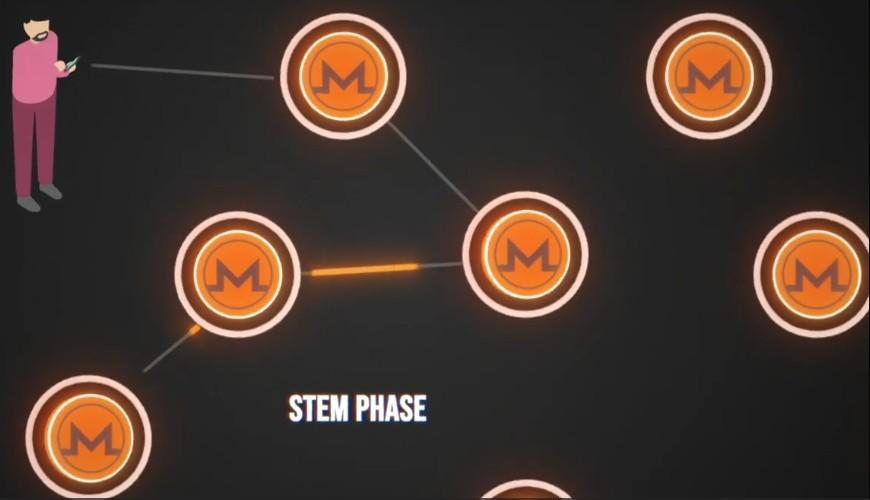
\includegraphics[scale=0.5]{images/stem-phase}
\end{figure}

The objective of the adversary is to increase the probability that
honest nodes connect to the spy nodes. They can do this by routing
traffic from leased IP addresses to their spy nodes. Honest nodes
routinely share the IP addresses of nodes with each other. Since the
Monero network is permissionless, spy nodes can simply share their
IP addresses with a few honest nodes. Then the spy node IP addresses
propagate throughout the network as honest nodes share peer IP addresses
with each other. See \cite{Cao2020} for more information on peer
list propagation. Honest nodes randomly select from their peer candidate
list when they drop old outbound connections and create new ones.

A subnet is a grouping of IP addresses. For example, a subnet with
256 IP addresses can be defined by setting the first three numbers
in dot-decimal notation to the same value, then having a distinct
number in the final position. Such a subnet could be all IP addresses
between \texttt{91.198.115.0} and \texttt{91.198.115.255}. This is
called a \texttt{/24} subnet because the first 24 bits of the IP address
are fixed, and the rest are allowed to vary. Another subnet that we
will discuss is the \texttt{/16} subnet, which follows a pattern of
\texttt{x.x.any.any}. Despite 16 being a smaller number than 24, a
\texttt{/16} subnet is much larger than a \texttt{/24} subnet, constituting
65,536 possible IP addresses instead of 256.

There are only about 4 billion possible IP addresses in the usual
IPv4 format. IPv6 addresses, which allow about $3.4\times10^{38}$
possible addresses, are disabled by default in the Monero node software
exactly because it would be too easy for an adversary to set up thousands
of IPv6 spy nodes cheaply.\footnote{See \href{https://libera.monerologs.net/monero/20230404\#c230903-c230904}{https://libera.monerologs.net/monero/20230404\#c230903-c230904}}
Where there is scarcity and demand, there is a market and therefore
a price. The limited IPv4 addresses are controlled by governments,
telecommunications companies, universities, and similar entities.
Some of these entities lease IP addresses on the open market. When
leasing in bulk, IP addresses are usually grouped into subnets. Some
brokers and lessors quote 118 to 250 USD per \texttt{/24} subnet per
month, which works out to 0.46 to 0.98 USD per IP address per month.\footnote{See \href{https://www.ipxo.com/lease-ips/}{https://www.ipxo.com/lease-ips/},
, \href{https://www.logicweb.com/bulk-ip-address-leasing/}{https://www.logicweb.com/bulk-ip-address-leasing/},
and \href{https://www.forked.net/ip-address-leasing/}{https://www.forked.net/ip-address-leasing/}}

Evidence uncovered by Monero developer boog900 suggests that a spy
node network is currently operating on the Monero network.\footnote{\href{https://github.com/monero-project/research-lab/issues/126}{https://github.com/monero-project/research-lab/issues/126}}
The spy node operator is leasing a combination of whole \texttt{/24}
subnets and individual IP addresses. As a temporary measure, the Monero
Research Lab has recommended that honest Monero node operators prevent
connections to the suspected spy node IP addresses by enabling a -{}\texttt{-ban-list}
option on their nodes.\footnote{See \href{https://github.com/monero-project/meta/issues/1124}{https://github.com/monero-project/meta/issues/1124}}
Enabling a ban list:
\begin{enumerate}
\item Requires node operators to trust the judgment and honesty of Monero's
developers and researchers,
\item Requires updating the IP address list if the adversary changes the
IP addresses it is leasing, and
\item Does not work against an adversary who deploys spy nodes that are
harder to distinguish from honest nodes.
\end{enumerate}
Therefore, a more universal solution is desired. Subnet deduplication
can counteract the adversary's bulk discount on leasing whole subnets.
First we will analyze the effect of subnet deduplication on the effectiveness
of the actual spy nodes currently deployed on the Monero network.
Then we will determine under what conditions subnet deduplication
is more effective than the status quo peer selection algorithm when
an adversary has free choice of whether to lease subnets or subnet-distinct
IP addresses.

\section{Simulated effect of subnet deduplication on current spy node effectiveness}

Monero's status quo peer selection algorithm does have one existing
countermeasure against spy node subnets. If Alice's node is already
connected to an IP address within a specific \texttt{/16} subnet,
then Alice's node will not connect to another node in that subnet.\footnote{\href{https://github.com/monero-project/monero/blob/84df77404e8bcbe1cf409f64c81e4e4f9c84885b/src/p2p/net_node.inl\#L1588}{https://github.com/monero-project/monero/blob/84df77404e8bcbe1cf409f64c81e4e4f9c84885b/src/p2p/net\_node.inl\#L1588}}
When an adversary leases many\texttt{ /24} subnets that are in distinct
\texttt{/16} subnets, this countermeasure is not very effective. Note
that the Tor protocol requires that no two nodes in its three-node
circuit can be in the same \texttt{/16} subnet \cite{Rochet2020}.

The proposed subnet deduplication peer selection algorithm keeps the
original rule about not selecting a peer that is in a \texttt{/16}
subnet that Alice is already connected to. In addition, it eliminates
from the peer candidate list all but one IP address in each \texttt{/16}
subnet. This form of the subnet deduplication algorithm is the most
aggressive. Less aggressive forms could deduplicate at a smaller subnet
level or keep more than one IP address in each subnet after deduplication.

To compare the effectiveness of spy nodes against the status quo algorithm
and the subnet deduplication algorithm, we must collect a list of
spy nodes, honest nodes, and their subnets. A list of IP addresses
accepting inbound connections for the Monero protocol can be obtained
easily by a Monero network scan.\footnote{\href{https://gist.github.com/Boog900/5e9fe91197fbbf5f5214df77de0c8cd8}{https://gist.github.com/Boog900/5e9fe91197fbbf5f5214df77de0c8cd8}}
First, the scanner contacts the Monero seed nodes to get an initial
list of nodes on the network. Then the scanner contacts all the nodes
on the initial list, requesting their own lists of nodes' IP addresses.
The scanner iterates through the accumulated list until all contactable
nodes have been contacted. These nodes can be classified into their
subnets and cross-referenced against the list of suspected spy nodes.

Figure \ref{fig-pre-dedup-treemap} plots a treemap of honest nodes
and spy nodes that accept inbound connections, based on a network
scan performed on February 11, 2025. Each of the 4,433 small colored
rectangles represents one node's IP address. Nodes in the same \texttt{/16}
subnet are grouped inside black-lined perimeters and are labeled with
white text where possible. Nodes in the same /24 subnet are grouped
inside yellow-lined perimeters. The share of the plot area that is
red is approximately the share of spy nodes on the network. Along
the left side and bottom of the plot, we observe six \texttt{/24}
subnets within distinct \texttt{/16} subnets that are entirely occupied
by spy nodes. Smaller numbers of spy nodes are scattered among \texttt{/16}
subnets that they share with some honest nodes, yet are in distinct
\texttt{/24} subnets (observe the yellow lines). These subnets are
likely owned by server providers used by honest nodes and spy nodes
alike. There are only two spy nodes alone in their own \texttt{/16}
subnets, but the majority of honest nodes are alone in their own \texttt{/16}
subnet.

\begin{figure}[H]
\caption{Subnet treemap of honest and spy nodes}

\label{fig-pre-dedup-treemap}

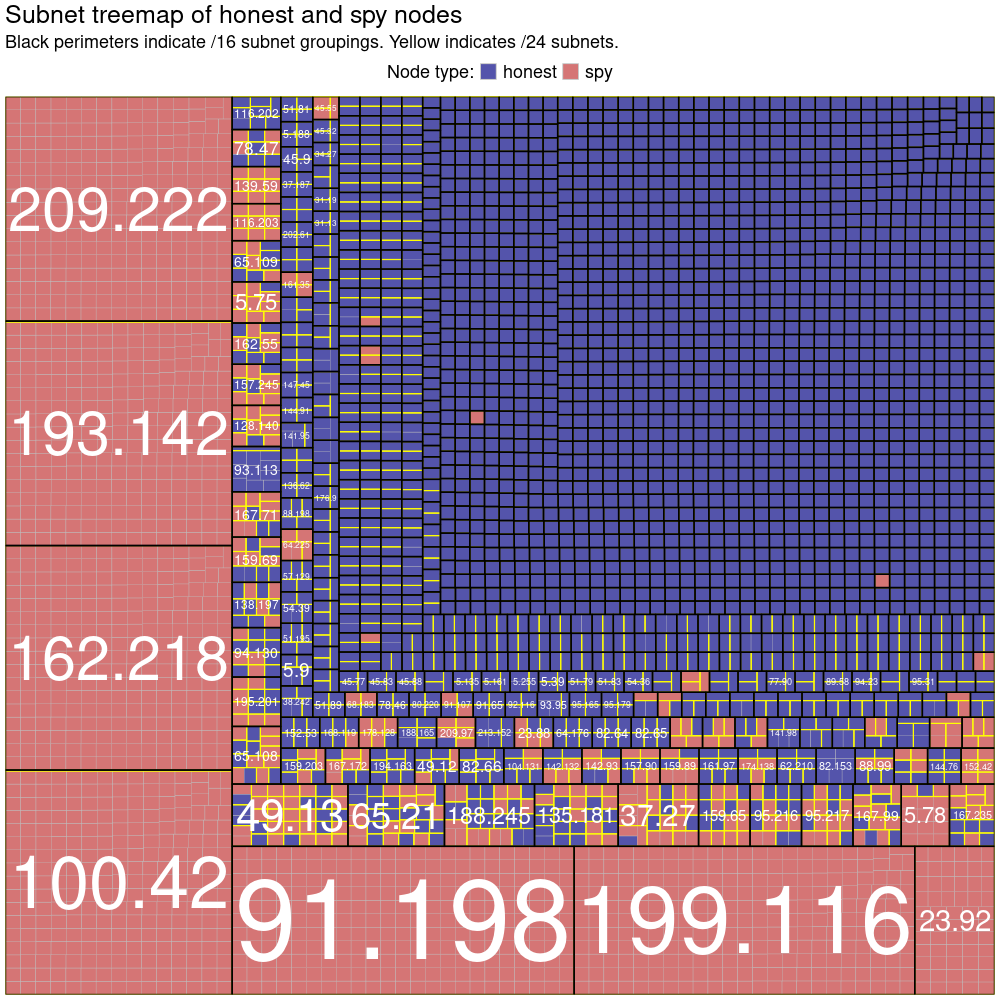
\includegraphics[scale=0.5]{images/treemap-status-quo}
\end{figure}

Figure \ref{fig-post-dedup-treemap} shows a treemap of honest nodes
and spy nodes after deduplication of \texttt{/16} subnets. When a
\texttt{/16} subnet contains both honest nodes and spy nodes, the
rectangle's color is a mixture of blue and red proportional to the
share of honest and spy nodes in the subnet. Compared to Figure \ref{fig-pre-dedup-treemap},
the area occupied by the red spy nodes is much smaller after subnet
deduplication.

\begin{figure}[H]
\caption{Subnet treemap of Honest and spy nodes after /16 subnet deduplication}

\label{fig-post-dedup-treemap}

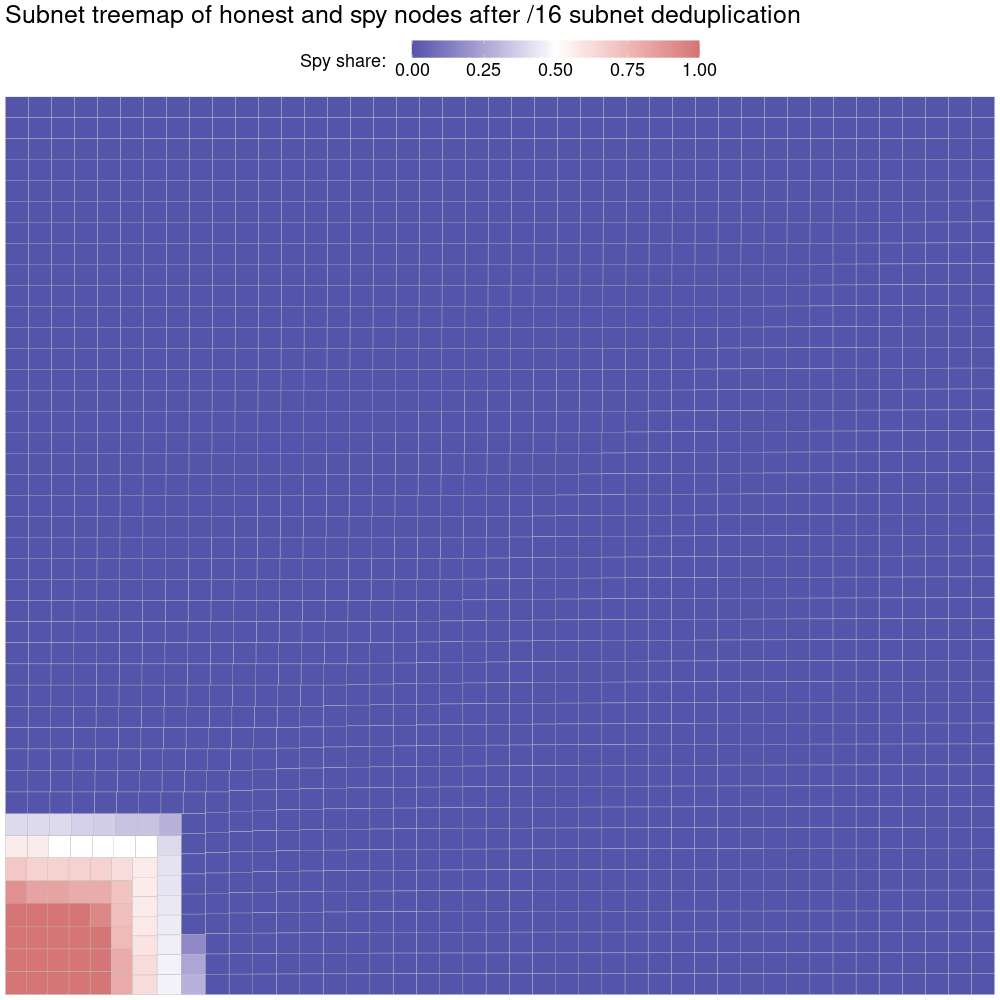
\includegraphics[scale=0.5]{images/treemap-16-subnet-deduplication}
\end{figure}

If each node chose a single peer node, then the share of connections
to spy nodes could be computed simply by dividing the total number
of nodes by the number of spy nodes. However, by default nodes choose
12 outbound peers without replacement. Probability computations where
elements are drawn without replacement with unequal probability are
known to be much more complicated than in problems where elements
are drawn with replacement with unequal probability \cite{TILLE2023100533}.
The computation is further complicated by the the status quo rule
to not select a peer in a \texttt{/16} subnet when already connected
to a peer in that \texttt{/16} subnet.

I wrote a Monte Carlo simulation that imitates the status quo and
subnet deduplication peer selection algorithms, using the data from
the network scan as its basis. First, the 12 outbound peer slots are
filled sequentially using the respective peer selection algorithm.
Then, peer ``churn'' is simulated 100 times. A churn occurs when
one peer is randomly dropped and a new one chosen, using the peer
selection rules. This simulation is done 10,000 times to estimate
the real share of a typical nodes's outbound peer connections that
would be composed of spy nodes. Note that the Monte Carlo simulation
ignores the fact that nodes' \texttt{white\_list} and \texttt{gray\_list}
are limited to 1,000 and 5,000 IP addresses, respectively. See \cite{Cao2020}
for more details about Monero's graylist housekeeping.

The results of the Monte Carlo simulation are as follows. When the
status quo peer selection algorithm is used, the share of connections
to spy nodes is 33.0 percent. When the subnet deduplication peer selection
algorithm is used, the share of connections to spy nodes is 2.5 percent. 

\section{Protocol-adversary interaction as a game}

Behavior is not static. When the actions of one agent change, other
agents may change their behavior, too. Therefore, we must go beyond
analyzing the effectiveness of subnet deduplication against a specific
adversary's current behavior. If the Monero protocol switches to subnet
deduplication, could privacy actually worsen? Can the cure be worse
than the disease? We will set up a simple game theory model and compute
under what conditions it is better to use the subnet deduplication
peer selection strategy. The theoretical result of this section is
that the choice of the honest node's strategy depends on the price
difference between bulk and individual IP address leasing, compared
to the concentration of honest nodes within subnets.

We make the following assumptions:
\begin{enumerate}
\item The privacy impact of spy nodes is equal to the probability of connecting
to a spy node in a single draw, with replacement. This ignores the
more complicated computations of drawing without replacement discussed
in the previous section.
\item Conditional on the pricing structure (i.e. bulk subnet or subnet-distinct
IP addresses), costs are a linear function of price. In other words,
if $w$ is the price and $x$ is the number of IP addresses leased,
then the cost is $w\cdot x$. This assumption may not be realistic
if the adversary exhausts low-cost IP address providers when leasing
a large number of IP addresses, and then must resort to high-cost
IP address providers.
\item The adversary is assumed to either lease only subnets or only subnet-distinct
IP addresses, i.e. no hybrid strategies. This assumption could be
relaxed in further work.
\end{enumerate}
There are two players, an honest node and a spying adversary. They
each can play two possible strategies. The honest node can use the
status quo peer selection algorithm or the subnet deduplication peer
selection algorithm. The adversary can lease whole \texttt{/24} subnets
at a bulk price discount or lease individual subnet-distinct IP addresses.
The game is assumed to be zero-sum. The payoff function for the adversary
is the probability that a single peer chosen by the honest node is
a spy node. The payoff function for the honest node is the negative
of that probability.

Define these probabilities that an honest node selects a spy node
peer:

$p_{s,s}$ when the honest node uses the status quo peer selection
algorithm and the adversary leases whole subnets,

$p_{d,s}$ when the honest node uses the subnet deduplication peer
selection algorithm and the adversary leases whole subnets,

$p_{s,d}$ when the honest node uses the status quo peer selection
algorithm and the adversary leases subnet-distinct IP addresses, and

$p_{d,d}$ when the honest node uses the subnet deduplication peer
selection algorithm and the adversary leases subnet-distinct IP addresses.

Table \ref{table-normal-form-game} shows the normal-form game. The
left side of each cell is the honest node's payoff. The right side
is the adversary's payoff.

\begin{table}

\caption{2x2 normal-form game}

\label{table-normal-form-game}

\begin{tabular}{|c|c|c|c|}
\cline{3-4} \cline{4-4} 
\multicolumn{1}{c}{} &  & \multicolumn{2}{c|}{Adversary}\tabularnewline
\cline{3-4} \cline{4-4} 
\multicolumn{1}{c}{} &  & Lease whole subnets & Lease subnet-distinct IP addresses\tabularnewline
\hline 
\multirow{2}{*}{Honest node} & Status quo & $-p_{s,s}$,$\quad$$p_{s,s}$ & $-p_{s,d}$,$\quad$$p_{s,d}$\tabularnewline
\cline{2-4} \cline{3-4} \cline{4-4} 
 & Subnet deduplication & $-p_{d,s}$,$\quad$$p_{d,s}$ & $-p_{d,d}$,$\quad$$p_{d,d}$\tabularnewline
\hline 
\end{tabular}

\end{table}

We want to know under what conditions will the honest node have more
privacy with a subnet deduplication peer selection algorithm instead
of the status quo peer selection algorithm. We assume that the adversary
uses the ``lease whole subnets'' strategy when the honest node uses
the status quo algorithm and the adversary uses the ``lease subnet-distinct
IP addresses'' strategy when the honest node uses the subnet deduplication
algorithm. Therefore, we want to know under what conditions $p_{s,s}>p_{d,d}$.

Let

$h_{s}$ be the total number of honest nodes that accept inbound connections,
including nodes in the same subnet,

$b$ be the budget of adversary,

$a$ be number of IP addresses leased by adversary, and

$w_{s}$ be the price per IP address when leasing whole subnets. (If
the price to lease a subnet is 150 USD, then the price per IP address
is 150/254 = 0.59 USD because there are 254 usable IP addresses in
a \texttt{/24} subnet.)

When using the status quo peer selection algorithm, the probability
that an honest node selects an adversary's IP address as a peer is
simply the share of nodes operated by the adversary:

$p_{s,s}=\dfrac{a}{h_{s}+a}$

How many adversary nodes exist? The adversary exhausts its budget,
so $a=b/w_{s}$. Now we have the probability that an honest node selects
an adversary's IP address as a peer in terms of the adversary's budget,
the price per leased IP address, and the number of honest nodes:

$p_{s,s}=\dfrac{b/w_{s}}{h_{s}+b/w_{s}}$

Multiplying through by $w_{s}$ gets us a simpler expression:

\begin{equation}
p_{s,s}=\dfrac{b}{w_{s}h_{s}+b}\label{eq:pss}
\end{equation}

$p_{s,s}$ denotes the probability that an honest node selects an
adversary's IP address when honest nodes are following the status
quo peer selection algorithm and the adversary is leasing whole subnets.
Next, we will compute $p_{d,d}$, the probability that an honest node
selects an adversary's IP address when honest nodes are following
a subnet deduplication peer selection algorithm and the adversary
is leasing IP addresses only in distinct subnets.

Let 

$h_{d}$ be the number of distinct subnets with at least one honest
node and

$w_{d}$ be the price to lease one subnet-distinct IP address.

By a similar logic as in the $p_{s,s}$ case,

\begin{equation}
p_{d,d}=\dfrac{b}{w_{d}h_{d}+b}\label{eq:pdd}
\end{equation}

Comparing (\ref{eq:pss}) and (\ref{eq:pdd}), it is easy to see that
$p_{s,s}>p_{d,d}$ if and only if $w_{s}h_{s}<w_{d}h_{d}$. Rearranging,
we have this condition:

\begin{equation}
\dfrac{w_{d}}{w_{s}}>\dfrac{h_{s}}{h_{d}}
\end{equation}

This inequality says that subnet deduplication is a better strategy
for the honest node if the price premium of leasing subnet-distinct
IP addresses is more than the ratio of the total number of honest
nodes to the number of distinct subnets with at least one honest node.
Note that this condition does not depend on the adversary's budget.

At any given moment, $h_{s}/h_{d}$ can be computed by performing
a network scan, assuming we can determine which nodes are honest.
Using the network scan and list of suspected spy nodes from the previous
section, we have $h_{s}/h_{d}=1.38$. That means that the subnet deduplication
algorithm is better than the status quo if the price premium to lease
subnet-distinct IP addreses is 38 percent or greater. Of course, the
subnet concentration of honest nodes can change over time.

\begin{singlespace}
\bibliographystyle{apalike-ejor}
\addcontentsline{toc}{section}{\refname}\bibliography{references}
\end{singlespace}

\end{document}
